%%%%%%%%%%%%%%%%%%%%%%%%%%%%%%%%%%%%%%%%%%%%%%%%%%%%%%%%%%%%%%%%%%%%%%%%%%%%%%%
% Uni Duesseldorf
% Lehrstuhl fuer Datenbanken and Informationssysteme
% Vorlage fuer Bachelor-/Masterarbeiten
% Optimiert fuer den Original-Latex-Kompiler LATEX.EXE (LaTeX=>PS=>PDF)
% Version 1.4 - 2.3.2010
%%%%%%%%%%%%%%%%%%%%%%%%%%%%%%%%%%%%%%%%%%%%%%%%%%%%%%%%%%%%%%%%%%%%%%%%%%%%%%%

%%%%%%%%%%%%%%%%%%%%%%%%%%%%%%%%%%%%%%%%%%%%%%%%%%%%%%%%%%%%%%%%%%%%%%%%%%%%%%%
%%%%%%%%%%% BEGINN EINSTELLUNG FUER DIE ARBEIT. UNBEDINGT ERFORDERLICH! %%%%%%%
%%%%%%%%%%%%%%%%%%%%%%%%%%%%%%%%%%%%%%%%%%%%%%%%%%%%%%%%%%%%%%%%%%%%%%%%%%%%%%%
% Geben Sie Ihren Namen hier an
\newcommand{\bearbeiter}{Alina Elterman}

% Geben Sie hier den Titel Ihrer Arbeit an
\newcommand{\titel}{Metrische Dimension Spezieller Graphklassen}

% Geben Sie das Datum des Beginns and Ende der Bachelorarbeit ein
\newcommand{\beginndatum}{28. Juni 2012}
\newcommand{\abgabedatum}{28. Dezember 2012}

% Geben Sie die Namen des Erst- and Zweitgutachters an
\newcommand{\erstgutachter}{Prof. Dr. Egon Wanke}
\newcommand{\zweitgutachter}{PD Dr. Frank Gurski}

% Falls Sie die Arbeit zweiseitig ausdrucken wollen,
% benutzen Sie die folgende Zeile mit
% \AN fuer zweiseitigen Druck
% \AUS fuer einseitigen Druck
\newcommand{\zweiseitig}{\AN}

% Falls die Arbeit in englischer Sprache verfasst 
% werden soll, dann benutzen Sie die folgende Zeile mit
% englisch fuer englische Sprache
% deutsch fuer deutsche Sprache
\newcommand{\sprache}{deutsch}
%%%%%%%%%%%%%%%%%%%%%%%%%%%%%%%%%%%%%%%%%%%%%%%%%%%%%%%%%%%%%%%%%%%%%%%%%%%%%%%%%
%%%%%%%%%%%%%%%%%%%%%%%%%%%%%%% ENDE EINSTELLUNGEN %%%%%%%%%%%%%%%%%%%%%%%%%%%%%%
%%%%%%%%%%%%%%%%%%%%%%%%%%%%%%%%%%%%%%%%%%%%%%%%%%%%%%%%%%%%%%%%%%%%%%%%%%%%%%%%%

% Die folgende Zeile NICHT EDITIEREN oder loeschen
% (Zum Ab�ndern der BA-Vorlage in eine MA-Vorlage muessen sie
% jedoch die Datei titelmakros1.tex selbst editieren.)
%%%%%%%%%%%%%%%%%%%%%%%%%%%%%%%%%%%%%%%%%%%%%%%%%%%%%%%%%%%
% Obere Titelmakros. Editieren Sie diese Datei nur, wenn
% Sie sich ABSOLUT sicher sind, was Sie da tun!!!
% (Z.B. zum Abaendern der BA-Vorlage in eine MA-Vorlage)
% Uni Duesseldorf
% Lehrstuhl fuer Datenbanken und Informationssysteme
% Version 2.2 - 2.3.2010
%%%%%%%%%%%%%%%%%%%%%%%%%%%%%%%%%%%%%%%%%%%%%%%%%%%%%%%%%%%
\newcommand{\AN}{twoside}
\newcommand{\AUS}{}
%\newcommand{\englisch}{}
%\newcommand{\deutsch}{\usepackage[german]{babel}}

%% Die folgenden auskommentierten Optionen dienen der automatischen
%% Erkennung des Latex-Kompilers und dem Setzen der davon abh�ngigen
%% Einstellungen. Bei Problem z.B. mit dem Einbinden von verschiedenen
%% Grafiktypen bei Verwendung von PdfLatex oder Latex, einfach die
%% verschiedenen \usepackage(s) ausprobieren. (Mit diesen Einstellungen
%% funktionierte diese Vorlage bei der Verwenundg von latex.exe als
%% Kompiler bei den meisten Studierenden.)

%\newif\ifpdf \ifx\pdfoutput\undefined
%\pdffalse % we are not running pdflatex
%\else
%\pdfoutput=1 % we are running pdflatex
%\pdfcompresslevel=9 % compression level for text and image;
%\pdftrue \fi

\documentclass[11pt,a4paper,pointlessnumbers, \zweiseitig]{scrreprt}



%\usepackage[iso]{umlaute}
%\usepackage[latin1]{inputenc}
\usepackage{palatino} % palatino Schriftart
%\usepackage{makeidx} % um ein Index zu erstellen
\usepackage{tocbibind}
\usepackage[T1]{fontenc} %fuer richtige Trennung bei Umlauten
\usepackage{fancybox} % fuer die Rahmen
\usepackage{shortvrb}
\usepackage{ifthen}
%\ifthenelse{\equal{\sprache}{deutsch}}{\usepackage[ngerman]{babel}}{}
\usepackage[utf8]{inputenc}
\usepackage{lmodern} 
\usepackage{amsmath}
\usepackage{oldgerm}
\usepackage{amssymb}
\usepackage{pdfpages}
\usepackage{hyperref}
%\usepackage{fancyheadings}
\usepackage{fancyhdr}
\usepackage{amsfonts}
\usepackage{amsthm}
\usepackage{color}
\usepackage{caption}
%\usepackage{stmaryrd}
\usepackage{graphicx}
\usepackage{graphics}
\usepackage{nomencl}
\usepackage[normalem]{ulem} 
\usepackage{verbatim}
\usepackage{ulsy}
\usepackage{floatflt}
\usepackage{float}
\usepackage{tikz}
\usepackage{pgf}
\usepackage{bbding}
\usepackage{nicefrac}
\usepackage{stmaryrd}
\usepackage{tabularx}
\usepackage{multirow}
\usepackage{array}
\usepackage{algorithm}
\usepackage{algorithmic}
% \usepackage[disable]{todonotes}				% alle todo-Anmerkungen ausblenden
\usepackage[german, color=yellow!40, colorinlistoftodos, textsize=footnotesize, shadow]{todonotes}
\usetikzlibrary{arrows,automata,petri,shapes,snakes}


\newcommand{\markup}[1]{\uline{#1}}
% Befehl umbenennen in abk
\let\abk\nomenclature

\usepackage{a4wide} % ganze A4 Weite verwenden

%\ifpdf
%\usepackage[pdftex,xdvi]{graphicx}
%\usepackage{thumbpdf} %thumbs fuer Pdf
%\usepackage[pdfstartview=FitV]{hyperref} %anklickbares Inhaltsverzeichnis
%\else
%\usepackage[dvips,xdvi]{graphicx}
%\usepackage{hyperref} %anklickbares Inhaltsverzeichnis
%\fi

%%%%%%%%%%%%%%%%%%%%%%% Massangaben fuer die Arbeit %%%%%%%%%%%%%%%
\setlength{\textwidth}{15cm}

\setlength{\oddsidemargin}{35mm}
\setlength{\evensidemargin}{25mm}

\addtolength{\oddsidemargin}{-1in}
\addtolength{\evensidemargin}{-1in}

%\makeindex
% Umgebungen f"ur S�tze usw.
\newtheorem{bem}{Bemerkung}
\newtheorem{definition}{Definition}
\newtheorem{bezeichnungen}{Bezeichnungen}
\newtheorem{fakt}{Fakt}
\newtheorem{beispiel}{Beispiel}
\newtheorem{bsp}{Beispiel}
\newtheorem{satz}{Satz}
\newtheorem{lem}{Lemma}
\newtheorem{idee}{Idee}
\newtheorem{corollary}{Korollar}
\floatname{algorithm}{Algorithmus}
\renewcommand{\algorithmicrequire}{\textbf{Eingabe:}}
\renewcommand{\algorithmicensure}{\textbf{Ausgabe:}}
\newenvironment{defi}[1][]{\ifthenelse{\equal{#1}{}}{\definition}{\definition[#1]}\rm}{\enddefinition}
\newcommand{\EP}[3]{
\medskip
\begin{center}
\begin{tabularx}{0.92\textwidth}{ll}
\hline\hline
\multicolumn{2}{c}{\textsc{#1}} \\
\hline
\em{Gegeben:}& #2\\
\em{Frage:}& #3 \\
\hline\hline
\end{tabularx}
\end{center}
\medskip}

\newcommand{\MP}[3]{
\medskip
\begin{center}
\begin{tabularx}{0.92\textwidth}{ll}
\hline\hline
\multicolumn{2}{c}{\textsc{#1}} \\
\hline
\em{Gegeben:}& #2\\
\em{Gesucht:}& #3 \\
\hline\hline
\end{tabularx}
\end{center}
\medskip}

%definition of new commands
\newcommand{\vsp}{\vspace{3mm}}
\newcommand{\impl}[1]{\overset{\text{#1}}{\implies}}
\newcommand{\notimplleft}[1]{\overset{\text{#1}}{\not\Leftarrow}}
\renewcommand{\figurename}{Abbildung}
\renewcommand{\tablename}{Tabelle}
\renewcommand{\contentsname}{Inhaltsverzeichnis}
\renewcommand{\listfigurename}{Abbildungsverzeichnis}
\renewcommand{\listtablename}{Tabellenverzeichnis}
\renewcommand\bibname{Literaturverzeichnis}
\begin{document}

%\setcounter{secnumdepth}{4} %Nummerieren bis in die 4. Ebene
%\setcounter{tocdepth}{4} %Inhaltsverzeichnis bis zur 4. Ebene

\pagestyle{headings}
\thispagestyle{empty}
\sloppy % LaTeX ist dann nicht so streng mit der Silbentrennung
%\MakeShortVerb{\�}

\parindent0mm
\parskip0.5em


{
\textwidth170mm 
\oddsidemargin30mm 
\evensidemargin30mm 
\addtolength{\oddsidemargin}{-1in}
\addtolength{\evensidemargin}{-1in}

\parskip0pt plus2pt

% Die Raender muessen eventuell fuer jeden Drucker individuell eingestellt
% werden. Dazu sind die Werte fuer die Abstaende `\oben' und `\links' zu
% aendern, die von mir auf jeweils 0mm eingestellt wurden.

%\newlength{\links} \setlength{\links}{10mm}  % hier abzuaendern
%\addtolength{\oddsidemargin}{\links}
%\addtolength{\evensidemargin}{\links}

\begin{titlepage}
\vspace*{-1.5cm}
  \raisebox{17mm}{
    \begin{minipage}[t]{70mm}
      \begin{center}
        %\selectlanguage{german}
        {\Large INSTITUT FÜR INFORMATIK\\}
        {\normalsize
          Algorithmen und Datenstrukturen
\\
        }
        \vspace{3mm}
        {\small Universitätsstr. 1 \hspace{5ex} D--40225 Düsseldorf\\}
     \end{center}
    \end{minipage}
  }
  \hfill
  \includegraphics[width=130pt]{HHU_Logo}
  \vspace{14em}

% Titel
  \begin{center}
      	\baselineskip=55pt
    	\textbf{\huge \titel}
  	 	\baselineskip=0 pt
   \end{center}

  %\vspace{7em}

\vfill

% Autor
  \begin{center}
    \textbf{\Large
      \bearbeiter
    }
  \end{center}

  \vspace{35mm}
 
% Pr�fungsordnungs-Angaben
  \begin{center}
    %\selectlanguage{german}
    
%%%%%%%%%%%%%%%%%%%%%%%%%%%%%%%%%%%%%%%%%%%%%%%%%%%%%%%%%%%%%%%%%%%%%%%%%
% Ja, richtig, hier kann die BA-Vorlage zur MA-Vorlage gemacht werden...
%%%%%%%%%%%%%%%%%%%%%%%%%%%%%%%%%%%%%%%%%%%%%%%%%%%%%%%%%%%%%%%%%%%%%%%%%
    {\Large Masterarbeit}

    \vspace{2em}

    \begin{tabular}[t]{ll}
      Beginn der Arbeit:& \beginndatum \\
      Abgabe der Arbeit:& \abgabedatum \\
      Gutachter:         & \erstgutachter \\
                         & \zweitgutachter \\
    \end{tabular}
  \end{center}

\end{titlepage}

}

%%%%%%%%%%%%%%%%%%%%%%%%%%%%%%%%%%%%%%%%%%%%%%%%%%%%%%%%%%%%%%%%%%%%%
%\clearpage
%\begin{titlepage}
%  ~                % eine leere Seite hinter dem Deckblatt
%\end{titlepage}
%%%%%%%%%%%%%%%%%%%%%%%%%%%%%%%%%%%%%%%%%%%%%%%%%%%%%%%%%%%%%%%%%%%%%
\clearpage
\begin{titlepage}
\vspace*{\fill}

\section*{Erklärung}

%%%%%%%%%%%%%%%%%%%%%%%%%%%%%%%%%%%%%%%%%%%%%%%%%%%%%%%%%%%
% Und hier ebenfalls ggf. BA durch MA ersetzen...
%%%%%%%%%%%%%%%%%%%%%%%%%%%%%%%%%%%%%%%%%%%%%%%%%%%%%%%%%%%

Hiermit versichere ich, dass ich diese Masterarbeit
selbstständig verfasst habe. Ich habe dazu keine anderen als die
angegebenen Quellen und Hilfsmittel verwendet.

\vspace{25 mm}

\begin{tabular}{lc}
Düsseldorf, den \abgabedatum \hspace*{2cm} & \underline{\hspace{6cm}}\\
& \bearbeiter
\end{tabular}

\vspace*{\fill}
\end{titlepage}

%%%%%%%%%%%%%%%%%%%%%%%%%%%%%%%%%%%%%%%%%%%%%%%%%%%%%%%%%%%%%%%%%%%%%
% Leerseite bei zweiseitigem Druck
%%%%%%%%%%%%%%%%%%%%%%%%%%%%%%%%%%%%%%%%%%%%%%%%%%%%%%%%%%%%%%%%%%%%%

%\ifthenelse{\equal{\zweiseitig}{twoside}}{\clearpage\begin{titlepage}
%~\end{titlepage}}{}

%%%%%%%%%%%%%%%%%%%%%%%%%%%%%%%%%%%%%%%%%%%%%%%%%%%%%%%%%%%%%%%%%%%%%
\clearpage
\begin{titlepage}

\section*{\ifthenelse{\equal{\sprache}{deutsch}}{Zusammenfassung}{Abstract}}


%%%%%%%%%%%%%%%%%%%%%%%%%%%%%%%%%%%%%%%%%%%%%%%%%%%%%%%%%%%%%%%%%%%%%%%%%%%%%%%%%
%%%%%%%%%%%%%%%%%%%%%%%%%%%% BEGINN ZUSAMMENFASSUNG %%%%%%%%%%%%%%%%%%%%%%%%%%%%%
%%%%%%%%%%%%%%%%%%%%%%%%%%%%%%%%%%%%%%%%%%%%%%%%%%%%%%%%%%%%%%%%%%%%%%%%%%%%%%%%%
Die metrische Dimension \ldots\\
1 SEITE
%%%%%%%%%%%%%%%%%%%%%%%%%%%%%%%%%%%%%%%%%%%%%%%%%%%%%%%%%%%%%%%%%%%%%%%%%%%%%%%%%
%%%%%%%%%%%%%%%%%%%%%%%%%%%%% ENDE ZUSAMMENFASSUNG %%%%%%%%%%%%%%%%%%%%%%%%%%%%%%
%%%%%%%%%%%%%%%%%%%%%%%%%%%%%%%%%%%%%%%%%%%%%%%%%%%%%%%%%%%%%%%%%%%%%%%%%%%%%%%%%

% Die folgende Zeile NICHT EDITIEREN oder loeschen
\input{titelmakros2}

%%%%%%%%%%%%%%%%%%%%%%%%%%%%%%%%%%%%%%%%%%%%%%%%%%%%%%%%%%%%%%%%%%%%%
%%%%%%%%%%%%%%%%%%%%%%%%% BEGINN TEXTTEIL %%%%%%%%%%%%%%%%%%%%%%%%%%%
%%%%%%%%%%%%%%%%%%%%%%%%%%%%%%%%%%%%%%%%%%%%%%%%%%%%%%%%%%%%%%%%%%%%%

%\listoftodos


\chapter{Einführung}
\begin{itemize}
\item BSP
\item Wo benutzt
\item Entwicklung der metrischen Dimension
\item Aufbau der Arbeit
\end{itemize}
%%%%%%%%%%%%%%%%%%%%%%%%%%%%%%%%%%%%%%%%%%%%%%%%%%%%%%%%%%%%%%%%%%%%%%%%%%%%%%%%%%%%%%%%%%%%%%%%%%%%%%%%%%%%%%%%
%%%%%%%%%%%%%%%%%%%%%%%%%%%%%%%%%%%%%%%%%%%%%%%%%%%%%%%%%%%%%%%%%%%%%%%%%%%%%%%%%%%%%%%%%%%%%%%%%%%%%%%%%%%%%%%%
%%%%%%%%%%%%%%%%%%%%%%%%%%%%%%%%%%%%%%%%%%%%%%%%%%%%%%%%%%%%%%%%%%%%%%%%%%%%%%%%%%%%%%%%%%%%%%%%%%%%%%%%%%%%%%%%

\begin{lem}
\label{sonneerweiterung}
Besteht ein Graph $G$ aus einem Kreis mit jeweils einem einfachen Weg an jedem Kreisknoten (Sonne aus Definition \ref{sun}). Auf jeder Kante auf dem Weg kann mit Knoten vom Grad zwei erweitert werden und Knoten von Grad zwei können ohne Auswirkungen auf die metrische Dimension kontrahiert werden.
\end{lem}
\begin{proof}[Beweis:]
Sei ein getrennter Kreis $G=(V,E)$ mit Wegen der Länge eins und seine metrische Basis $R$ gegeben. Eine Kante auf einem Weg an Knoten $v_k$ wird um einen Knoten erweitert, so dass sich die metrischen Koordinaten von Knoten $v$, welcher kein Ankerknoten ist, um eins erhöhen. Sei $a+2/b+2$ für einen ungeraden Kreis und $a+2/b+2/c+2$ für einen geraden Kreis die neuen metrischen Koordinaten von $v$. Angenommen, es gibt einen Knoten $u$ in dem Graphen $G$ mit den gleichen metrischen Koordinaten.
\begin{enumerate}
\item Der Knoten $v_k$ hat die metrischen Koordinaten $a/b$ oder $a/b/c$. Sofern es einen anderen Knoten $v'$ als $v$ gibt mit der Distanz zwei zu dem Knoten $v_k$ und den gleichen metrischen Koordinaten wie $v$, so gibt es auch einen Knoten zwischen den Knoten $v'$ und $v$ mit den metrischen Koordinaten $a+1/b+1$ oder $a+1/b+1/c+1$. Dieser Knoten hat die gleichen metrischen Koordinaten wie der Knoten $v$ vor der Erweiterung. Dadurch hätte der ursprüngliche Graph nicht getrennt sein können.
\item Angenommen, es gibt einen Knoten $v'$ als $v$ mit der Distanz $2a+2$ zu dem Knoten $v_k$ und den gleichen metrischen Koordinaten wie $v$.
\begin{itemize}
\item Der Knoten $v'$ liegt auf dem Kreis.
\begin{itemize}
\item Ist der Kreis ungerade, so kann die metrische Koordinate bzgl. des zweiten Ankerknotens $b+2$ sein wenn der kürzeste Weg von beiden Ankerknoten von $v_k$ nach $v'$ gleich ist. Damit hätten beide Ankerknoten den gleichen Bifurkator und damit tritt Fall 1 ein.
Oder die metrische Koordinate ist $b-b+2n+1-2a-2=2(n-a)-1$. Dieser Wert ist für alle $a,b,n \in \mathbb{N}$ ungerade und damit insbesondere $2(n-a)-1\neq 2b+2$. 
\item Ist der Kreis gerade, so können die metrischen Koordinaten gleich sein, wenn zwei Ankerknoten im gleichen Strahl sind. Ist das der Fall, so wäre auch der ursprüngliche Graph nicht getrennt. Ausgenommen von diesem Strahl werden dieselben Knotenpaare von beide Ankerknoten getrennt, und nach Lemma \ref{} reichen zwei Ankerknoten nicht aus um einen geraden Sonnengraphen zu trennen. Sind alle Knoten in unterschiedlichen Strahls, so kann es keine zwei Knoten mit einer Distanz $\geq \frac{n}{2}$ geben, so dass alle drei Markierungen gleich sind.
\end{itemize}
\item Der Knoten $v'$ ist ein Blatt. 
\begin{itemize}
\item Dann gibt es einen Strahlursprung $v'_k$ mit der Distanz eins zu dem Knoten $v'$ und mit der Distanz $2a+1$ zu dem Knoten $v_k$. Angenommen die Ankerknoten haben keinen gemeinsamen Bifurkator, dann hat $v'$ die metrische Korrdinate $b-b+2n-2a-1=2(n-a)$. Dieser Wert ist für alle $a,b,n \in \mathbb{N}$ gerade und damit auch $2(n-a)\neq 2b+1$.
\item In einem geraden Sonnengraphen kann es keine zwei Knoten geben, so dass die Distanz von drei Ankerknoten zu diesen beiden Knoten gleich ist. Ausgenommen mindestens zwei Knoten liegen aus einem Strahl.
\end{itemize}
\end{itemize}
\end{enumerate}
\end{proof}
%%%%%%%%%%%%%%%%%%%%%%%%%%%%%%%%%%%%%%%%%%%%%%%%%%%%%%%%%%%%%%%%%%%%%%%%%%%%%%%%%%%%%%%%%%%%%%%%%%%%%%%%%%%%%%%%
%%%%%%%%%%%%%%%%%%%%%%%%%%%%%%%%%%%%%%%%%%%%%%%%%%%%%%%%%%%%%%%%%%%%%%%%%%%%%%%%%%%%%%%%%%%%%%%%%%%%%%%%%%%%%%%%
%%%%%%%%%%%%%%%%%%%%%%%%%%%%%%%%%%%%%%%%%%%%%%%%%%%%%%%%%%%%%%%%%%%%%%%%%%%%%%%%%%%%%%%%%%%%%%%%%%%%%%%%%%%%%%%%
\chapter{Metrische Dimension von kreisähnlichen Graphklassen}
\vspace{-3mm}
In diesem Kapitel geht es um Erweiterungen von bekannten Graphklassen.\\Als erstes werden der Freundschaftsgraph und seine Verallgemeinerung und dannach der Sonnengraph inkl. der unvollständigen Variante untersucht.
Von den verallgemeinerten Freundschaftsgraphen und beiden Sonnengraphen wird die metrische Dimension bestimmt unter der Vorraussetzung, dass ein Teil der metrischen Basis fest vorgegeben ist. Die Resultate werden bei dem Algorithmus zur Bestimmung der metrischen Dimension von Kaktusgraphen in Kapitel \ref{kapkaktus} und bei dem Beweis der metrischen Dimension der $C_j-$Bäume in Kapitel \ref{kapcjbaume} benötigt.
\vspace{-4mm}
\section{Metrische Dimension der Freundschaftsgraphen $F_{n}$}
''Haben je zwei Bekannte einen weiteren gemeinsamen Bekannten und sie sind untereinander bekannt, so gibt es eine Person, welche alle anderen kennt''. Diese Behauptung kann als ein Graphenproblem definiert werden, wobei Knoten Personen und Kanten Bekannschaften repräsentieren. Um es zu lösen wurde von Paul Erdős et al. \cite{Erdos} der Freundschaftsgraph eingeführt. In der Arbeit von Baskoro et. al \cite{amal} wird die metrische Dimension von den Freundschaftgraphen bestimmt. Der Schwerpunkt dieser Arbeit liegt auf der Anzahl der unterschiedlichen metrischen Basen.
\begin{defi}{\textbf{(Freundschaftsgraph $F_{n,3}$)}}\\
Der Freundschaftsgraph $F_{n,3}=(V,E)$ besteht aus der Knotenmenge $$V = \{u,v_{1,1},v_{1,2},v_{2,1},v_{2,2},\ldots,v_{n,1},v_{n,2}\}$$ und der Kantenmenge $$E = \{ \{u,v_{1,i}\}~|~ 1 \leq i \leq n \} \cup \{ \{u,v_{i,2}\}~|~ 1 \leq i \leq n \} \cup \{ \{ v_{i,1}, v_{i,2} \} ~|~ 1 \leq i \leq n \}$$
Die Kanten $\{u,v_{i,1}\},\;\{u,v_{i,2}\}$ und $\{v_{i,1},v_{i,2}\}$ bilden den $i$-ten Kreis $C_3$.
\end{defi}
\begin{bsp}~
\vspace{-3mm}
\begin{figure}[h!]
\centering
 		 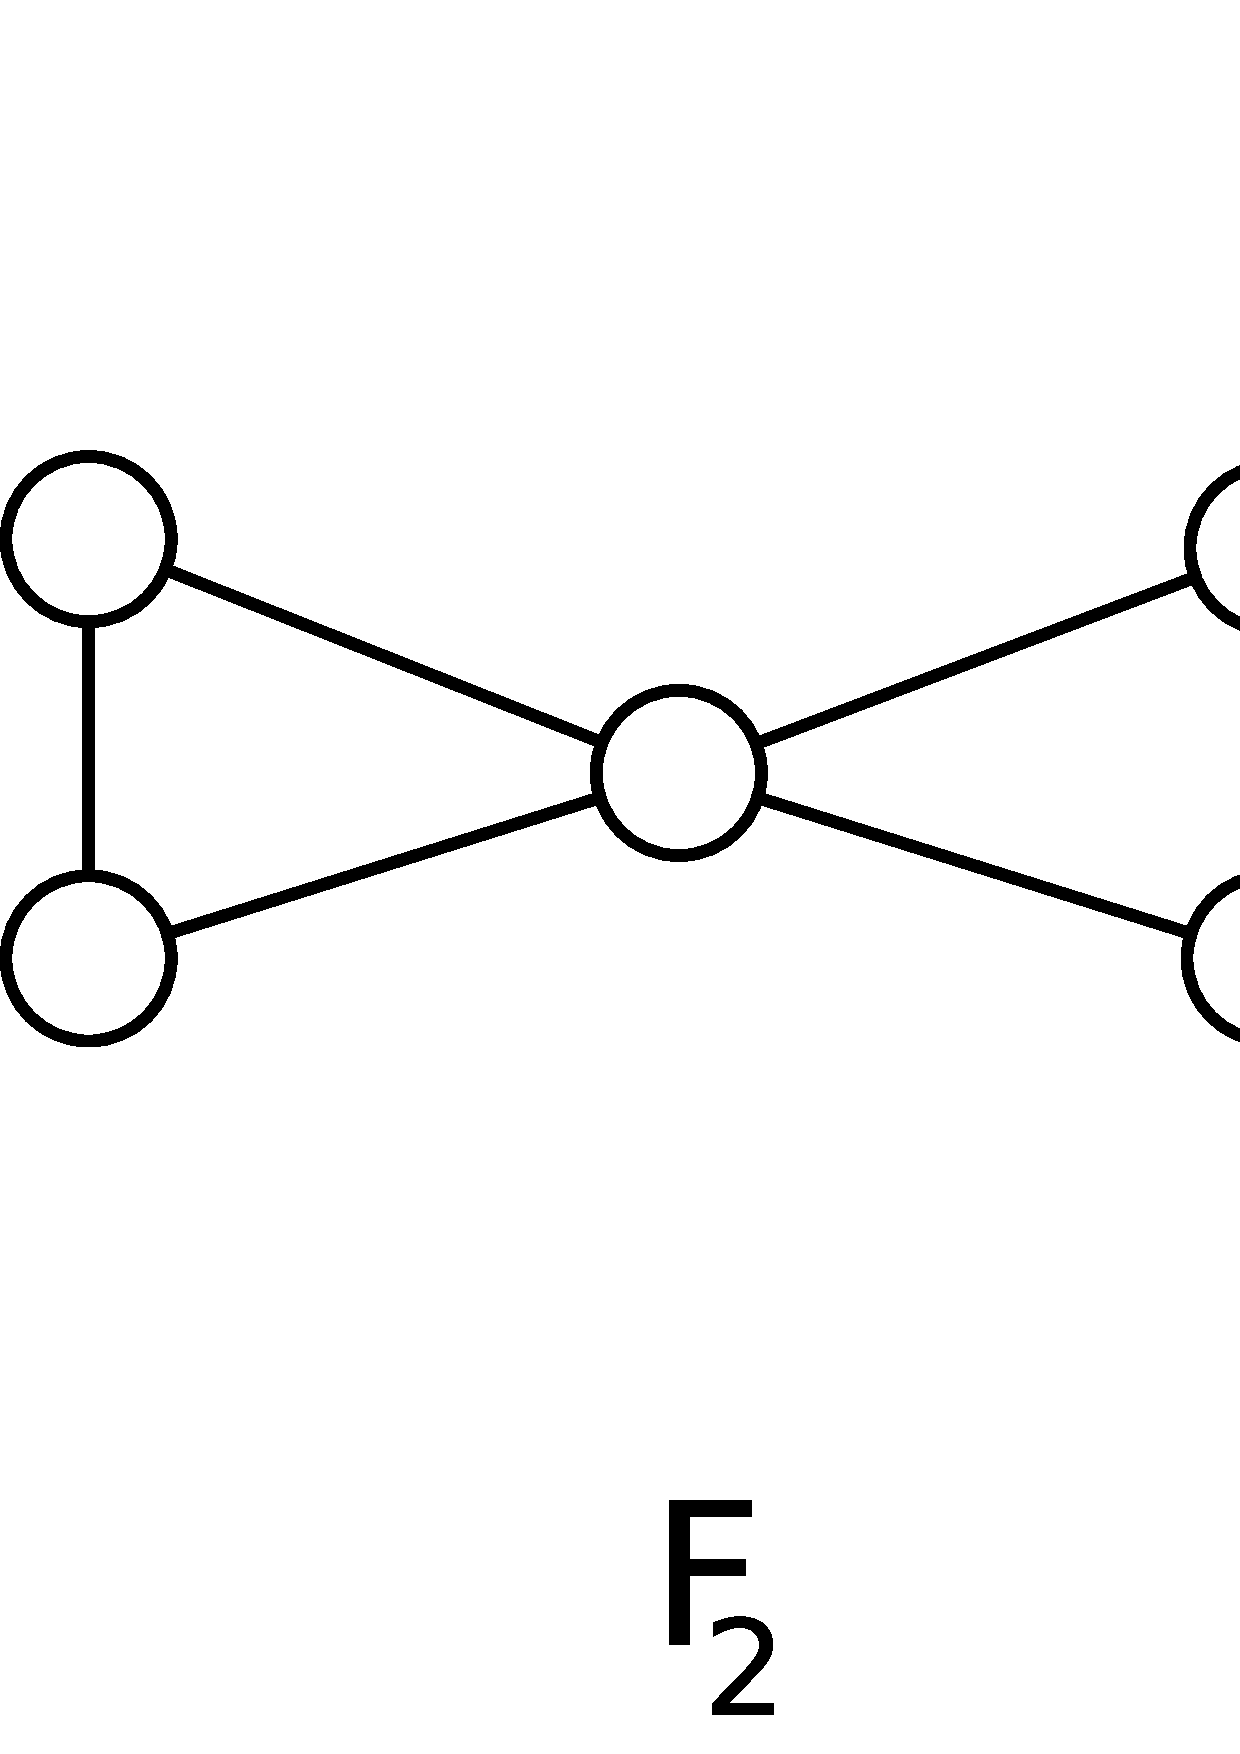
\includegraphics[width=380pt]{bilder/freunschaftsgraph.pdf}
   \caption{Vier Freundschaftsgraphen}
   \label{bild:fg}
\end{figure}
\end{bsp}\newpage
\begin{lem}
\label{Freundschaftsgraphen}
Die metrische Dimension eines Freundschaftsgraphen $F_{n,3}$ ist $n$.
\end{lem}
Um diese Behauptung zu beweisen, wird das folgende Lemma benötigt. 
\begin{lem}
\label{mindfreundschaftsgraph}
Sei ein Freundschaftsgraph $F_{n,3}$ gegeben. Jede metrische Basis muss aus dem $i$-ten $C_3$ mindestens einen der folgenden Knoten $\{v_{i,1},v_{i,2}\}$ beinhalten. 
\end{lem}
\vspace{-2mm}
\begin{proof}[Beweis:]~
\par
\begin{floatingfigure}[l]{200pt}
{\flushleft
\hspace*{1.7cm}
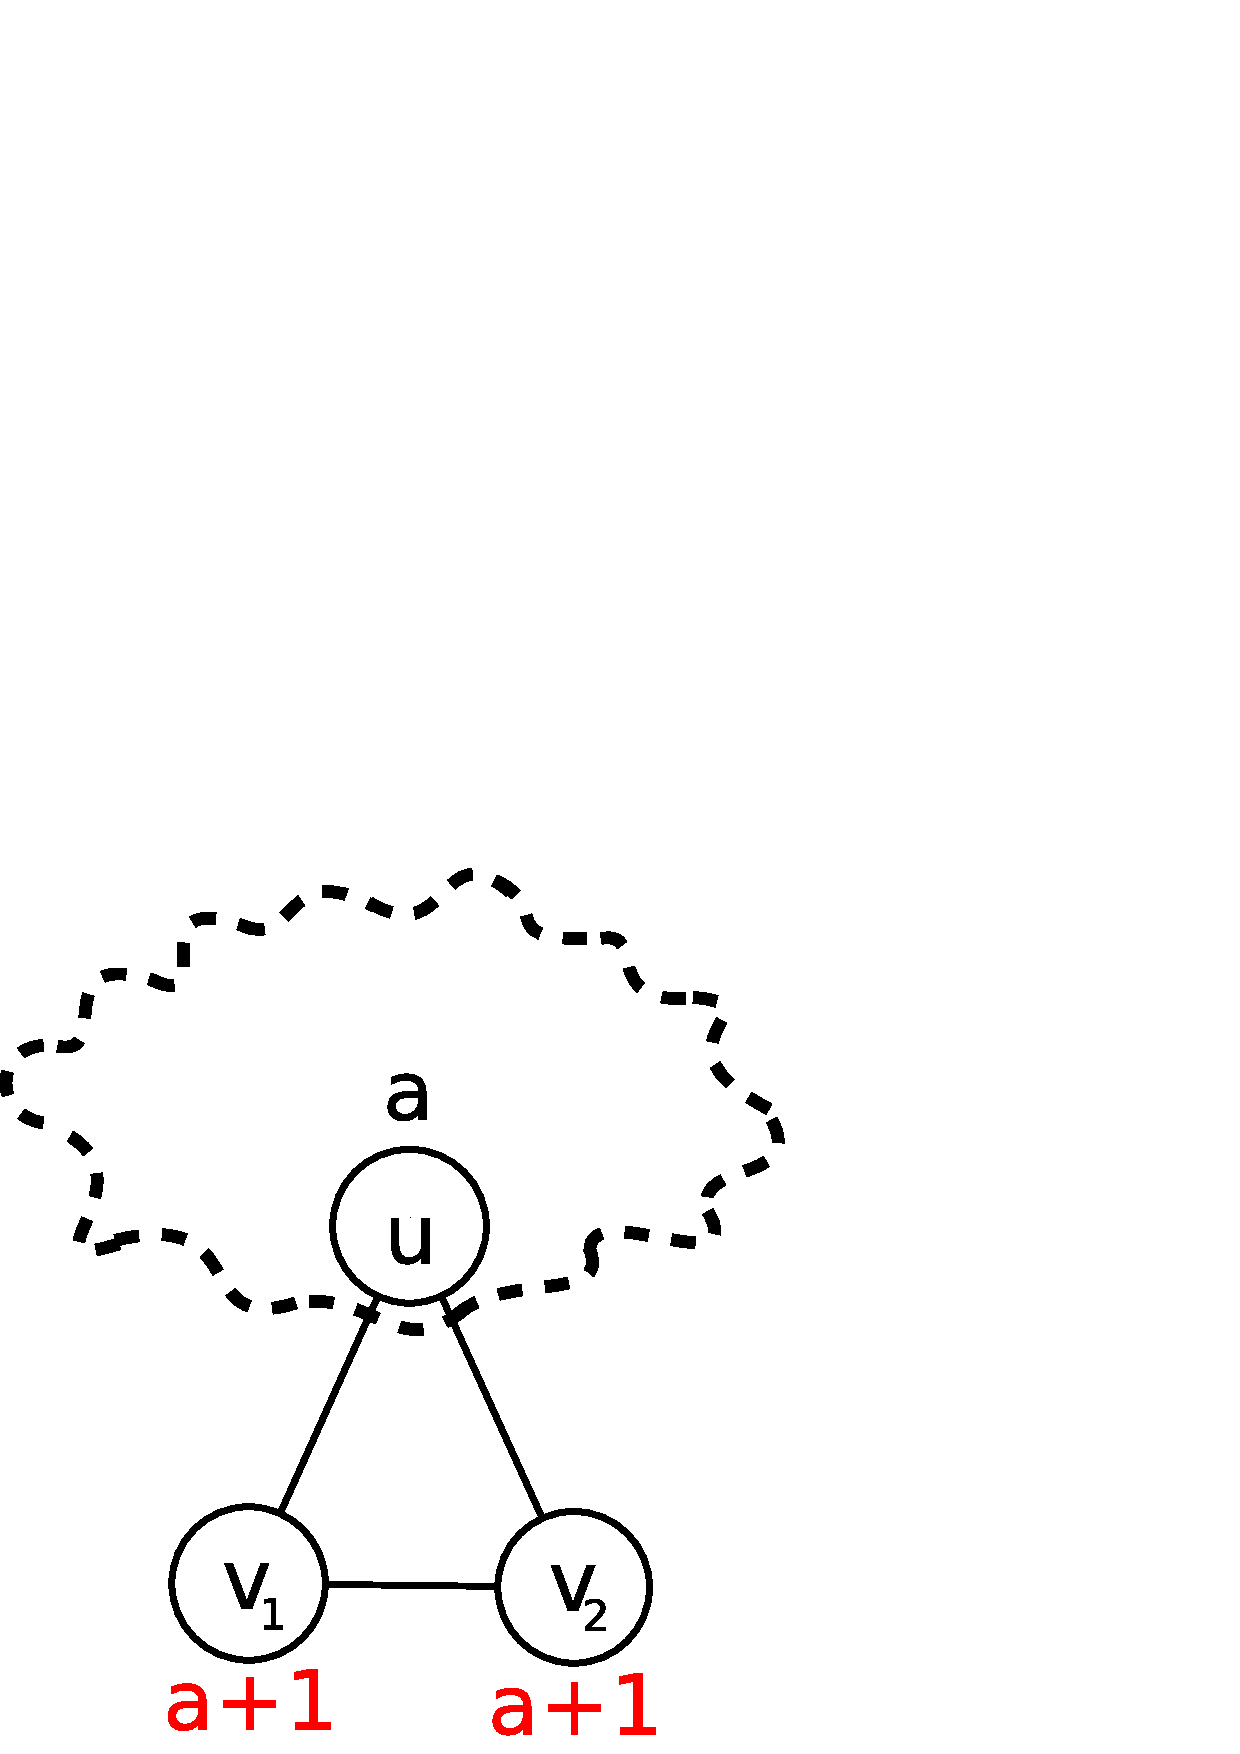
\includegraphics[width=100pt]{bilder/freundschaftsgraphbew.pdf}}
\caption{Ein markierter $C_{3}$}
\label{CA9}
\end{floatingfigure}

Angenommen es gibt einen $C_3$ ohne Ankerknoten. Durch die eindeutige Verbindung zu dem Restgraphen, welche über einen\\Trennungsknoten läuft, folgt aus Symmetriegründen, dass die Knoten $v_{i,1}$ und $v_{i,2}$ identische Markierungen haben.\\Dies ist ein Widerspruch zu der Definition einer metrischen Basis.\\
Die metrische Dimension eines Freundschaftsgraphen $F_{n,3}$ ist mindestens gleich der Anzahl seiner $C_{3}$, mindestens $n$.
\end{proof}
\par
\vspace{-2mm}
\begin{proof}[Beweis von Lemma \ref{Freundschaftsgraphen}:] \vspace{+1mm} ~ \linebreak
Nach Lemma \ref{mindfreundschaftsgraph} ist bekannt, dass die metrische Dimension eines Freundschaftsgraphen $F_{n,3}$ mindestens $n$ ist. Angenommen, alle als $v_{2,i}$ markierten Knoten werden in die metrische Basis aufgenommen. Also sind sie getrennt. Der Knoten $v_1$ hat die Distanz eins zu allen Knoten in der metrischen Basis und ist der einzige Knoten mit dieser Eigenschaft. Für jeden Knoten $v_{3,i}$ gibt es genau einen Knoten $v_{2,i}$ mit der Distanz eins. Zu allen anderen Knoten in der metrischen Basis hat jeder Knoten $v_{3,i}$ die Distanz zwei. Alle Markierungen sind eindeutig und der gesamte Graph ist durch die $n$ Knoten getrennt.
\end{proof}
\vspace{-14mm}
~ \linebreak
\begin{defi}{\textbf{(Freundschaftsgraph $F_n$)}}\\
%Der $k$-fache Freundschaftsgraph $F_{n,k}=(V,E)$ mit $k\geq 3$ besteht aus der Knotenmenge $$V = \{u,v_{1,1}, \ldots, v_{1,k-1},v_{2,1},\ldots v_{2,k-1},\ldots,v_{n,1},\ldots v_{n,k-1}\}$$ und der Kantenmenge $$E = \{ \{u,v_{1,i}\}~|~ 1 \leq i \leq n \} \cup \{ \{u,v_{i,k-1}\}~|~ 1 \leq i \leq n \}$$$$\cup \{ \{ v_{i,j}, v_{i,j+1} \} ~|~ 1 \leq i \leq n \text{ und }1 \leq j \leq k-2\}$$
Der Freundschaftsgraph $F_{n}=(V,E)$ mit $k_1,\ldots, k_n \geq 3 $ besteht aus der Knotenmenge $$V = \{u,v_{1,1}, \ldots, v_{1,k_1-1},v_{2,1},\ldots v_{2,k_2-1},\ldots,v_{n,1},\ldots v_{n,k_n-1}\}$$ und der Kantenmenge $$E = \{ \{u,v_{1,i}\}~|~ 1 \leq i \leq n \} \cup \{ \{u,v_{i,k_i-1}\}~|~ 1 \leq i \leq n \}$$$$\cup \{ \{ v_{i,j}, v_{i,j+1} \} ~|~ 1 \leq i \leq n \text{ und }1 \leq j \leq k_i-2\}$$
Die Kanten $\{u,v_{i,1}\},\;\{u,v_{i,k-1}\}$ und $\{v_{i,j},v_{i,j+1}\}$ für $1 \leq j \leq k_i-2$ bilden den $i$-ten Kreis $C_k$.
\end{defi}

\begin{lem} \cite{amal}
\label{verallgFreundschaftsgraphen}
Die metrische Dimension eines Freundschaftsgraphen $F_{n}$ mit $t_1$ Kreisen der Länge $k=2j+1$ für $j \geq 1$ und $t_2$ Kreisen der Länge $k=2j$ für $j \geq 2$ ist 
\begin{equation}
   \beta(F_{n,k})=
   \begin{cases}
     t_1 & \text{f\"ur } t_2=0 \\
     2\cdot t_2-1 & \text{f\"ur } t_1=0 \\
     t_1+ 2\cdot t_2-1 & sonst
   \end{cases}
\end{equation}
\end{lem}
\begin{lem}
Beinhaltet ein Freundschaftgraph mindestens ein gerades $k_i$ und ist $n\geq 2$, so beinhaltet jede metrische Basis mindestens zwei Knoten aus jedem $i$-ten Kreis mit einem geraden $k_i$.  
\end{lem}
\subsection{Metrische Dimension von allgemeinen Freundschaftgraphen und Bäumen}
\label{amal}
%%%%%%%%%%%%%%%%%%%%%%%%%%%%%%%%%%%%%%%%%%%%%%%%%%%%%%%%%%%%%%%%%%%%%%%%%%%%%%%%%%%%%%%%%%%%%%%%%%%%%%%%%%%%%%%%
\newpage
\section{Metrische Dimension der Sonnengraphen $S_{n,k}$}
\label{chap_sonne}
In der Arbeit ''The metric dimension of graph with pendant edges'' \cite{sun} betrachteten Baskoro et. al. die metrische Dimension des Corona Produktes von Kreisen $C_n$ und Wegen $P_1$. In diesem Kapitel wird gezeigt, dass ihr Resultat sich auf Wege beliebiger Länge übertragen lässt. Außerdem werden ebenfalls Teilgraphen der Sonnengraphen betrachtet, die unvollständigen Sonnengraphen. Diese Graphklasse ist sehr wichtig, denn beide Variationen von Sonnengraphen sind induzierte Teilgraphen von den in Kapitel \ref{kapcjbaume} behandelten $C_j$-Bäumen und den in Kapitel \ref{kapkaktus} behandelten Kaktusgraphen.
\begin{defi}{\textbf{(Sonnengraph $S_{n}$)}}\\
\label{sun}
Sei ein Kreis $C_n$ für $n \geq 3$ mit der Knotenmenge $|V|=\{ c_1, \ldots , c_n \}$ und $n$ Weggraphen $P_{k-1}$ für $k \geq 2$ gegeben. Die Knoten mit Grad eins auf dem $i-$ten Weg werden als $v_{i,1}$ und $v_{i,k-1}$ bezeichnet. Durch das Hinzufügen von $n$ neuen Kanten der Form $\{v_{i,1},c_i\}$ für $1 \leq i \leq n$ ensteht der zusammenhängende Sonnengraph $S_{n,k}$.\\
Alle als $v_{i,k-1}$ bezeichneten Knoten werden Endknoten genannt, als $c_i$ bezeichnete Knoten werden Ursprungsknoten genannt und eine Knotenmenge mit den Knoten $\{c_i,v_{i,1}, \ldots ,v_{i,k-1}\}$ für $1 \leq i \leq n$ als Strahl. (vgl. Abbildung \ref{bild:sonnengraph})\\
Für $n=1$ ist der Graph der Sterngraph aus Definition \ref{defstern}. Als Sonnengraph $S_n$ bezeichne man einen Graphen mit $n$ Strahlen beliebiger Länge $i$ mit $i \geq 2$.
\end{defi}
\begin{figure}[h!]
\centering
 		 \includegraphics[width=165pt]{bilder/sonne4.pdf}
   \caption{Der Sonnengraph $S_{12,3}$}
   \label{bild:sonnengraph}
\end{figure}
%\begin{bem}
%Nach Satz \ref{sepvertex} können beliebige Wege $P_i$ mit $i\geq 2$ bei der Berechnung der metrischen Dimension als $P_2$ aufgefasst werden. Also gilt: $$md(S_{n,2})=md(S_{n,3})= \ldots =md(S_{n,k})=md(S_{n})$$
%Im folgenden wird der Graph $S_{n,2}$ repräsentativ für $S_{n,k}$ betrachtet.
%\end{bem}
\begin{lem}\cite{sun}
\label{sun1}
Für die metrische Dimension eines Sonnengraphen $S_{n,1}$ gilt:
\begin{equation}
   \beta(S_{n,1})=
   \begin{cases}
     2 & \text{f\"ur } n = 4 \text{ oder } n = 2j+1 \text{ f\"ur } j \in \mathbb{N} \\
     3 & \text{f\"ur } n = 2j+4 \text{ f\"ur } j \in \mathbb{N} 
   \end{cases}
\end{equation}
\end{lem}
\begin{lem}
\label{knotenimstrahl}
Es gibt pro Strahl nur einen Ankerknoten. Das Vorziehen eines Endknotens gegenüber einem Strahlurprung als Ankerknoten im gleichen Strahl bringt nur Vorteile.
\end{lem}
\begin{proof}[Beweis:]
Angenommen der Endknoten eines Strahls ist ein Ankerknoten $r$. Der Bifurkator zwischen jedem Knoten auf dem Strahl und einem beliebigen Knotenpaar im restlichen Graphen ist der Strahlursprung. Der Strahlurprung ist ebenfalls der Bifurkator für den Ankerknoten und jedem Knotenpaar im Graphen außerhalb des Strahls. Nach Lemma \ref{bifur} ist jeder Knoten auf dem Strahl damit kein zusätzlicher Ankerknoten. Jeder Knoten auf dem Strahl ist im gesammten Graphen getrennt, da er durch einen Weg eine eindeutige Distanz zu dem Ankerknoten $r$ hat.\begin{figure}[h!]
		\centering
 		 \includegraphics[width=300pt]{bilder/bspsonne4.pdf}
   \caption{$S_4$ mit zwei Ankerknoten unterschiedlich positioniert}
   \label{s4}
   \end{figure}
Nimmt man in einem Strahl den Strahlursprung an Stelle des Endknotens so kann ein getrennter Graph nicht nicht mehr getrennt sein. (vgl. dazu Abbildung \ref{s4})
\end{proof}
%Es werden nur noch metrische Basen betrachtet mit maximal einem Ankernoten in einem Strahl. Das Auswirkungen von Lemma \ref{sonneerweiterung}, dass für die Bestimmung der metrischen Dimension einer Sonne $S_n$ einfach die metrische Dimension einer Sonne $S_{n,1}$ bestimmt werden kann. 
\begin{bem}
Es werden nur noch metrische Basen mit maximal einem Ankernoten in einem Strahl betrachtet. O.B.d.A. ist der Endknoten des Strahls der Ankerknoten. Außerdem gilt nach Lemma \ref{sonneerweiterung} für die metrische Dimension von Sonnengraphen: $$\beta(S_{n,1})=\beta(S_{n,k})=\beta(S_n)$$
Dadurch wird bei der weiteren Berechnung nur der Sonnengraph $S_{n,1}$ beachtet, da sich die Ergebnisse auf jeden beliebigen Sonnengraph übertragen lassen. 
\end{bem}
\begin{lem}
Die metrische Dimension eines Sonnengraphen $S_{n}$ mit $n = 2j+4$ für $j \in \mathbb{N}^+$ ist größer als zwei. 
\end{lem}
%\begin{figure}[h!]
%\begin{minipage}[hbt]{7cm}
%	\centering
%	\includegraphics[width=170pt]{bilder/sonne4k.pdf}  
 %  \caption{Der Sonnengraph $S_{4,2}$}  
	%\label{Bild1}
%\end{minipage}
%\hfill
%\begin{minipage}[hbt]{7cm}%
%	\centering
%	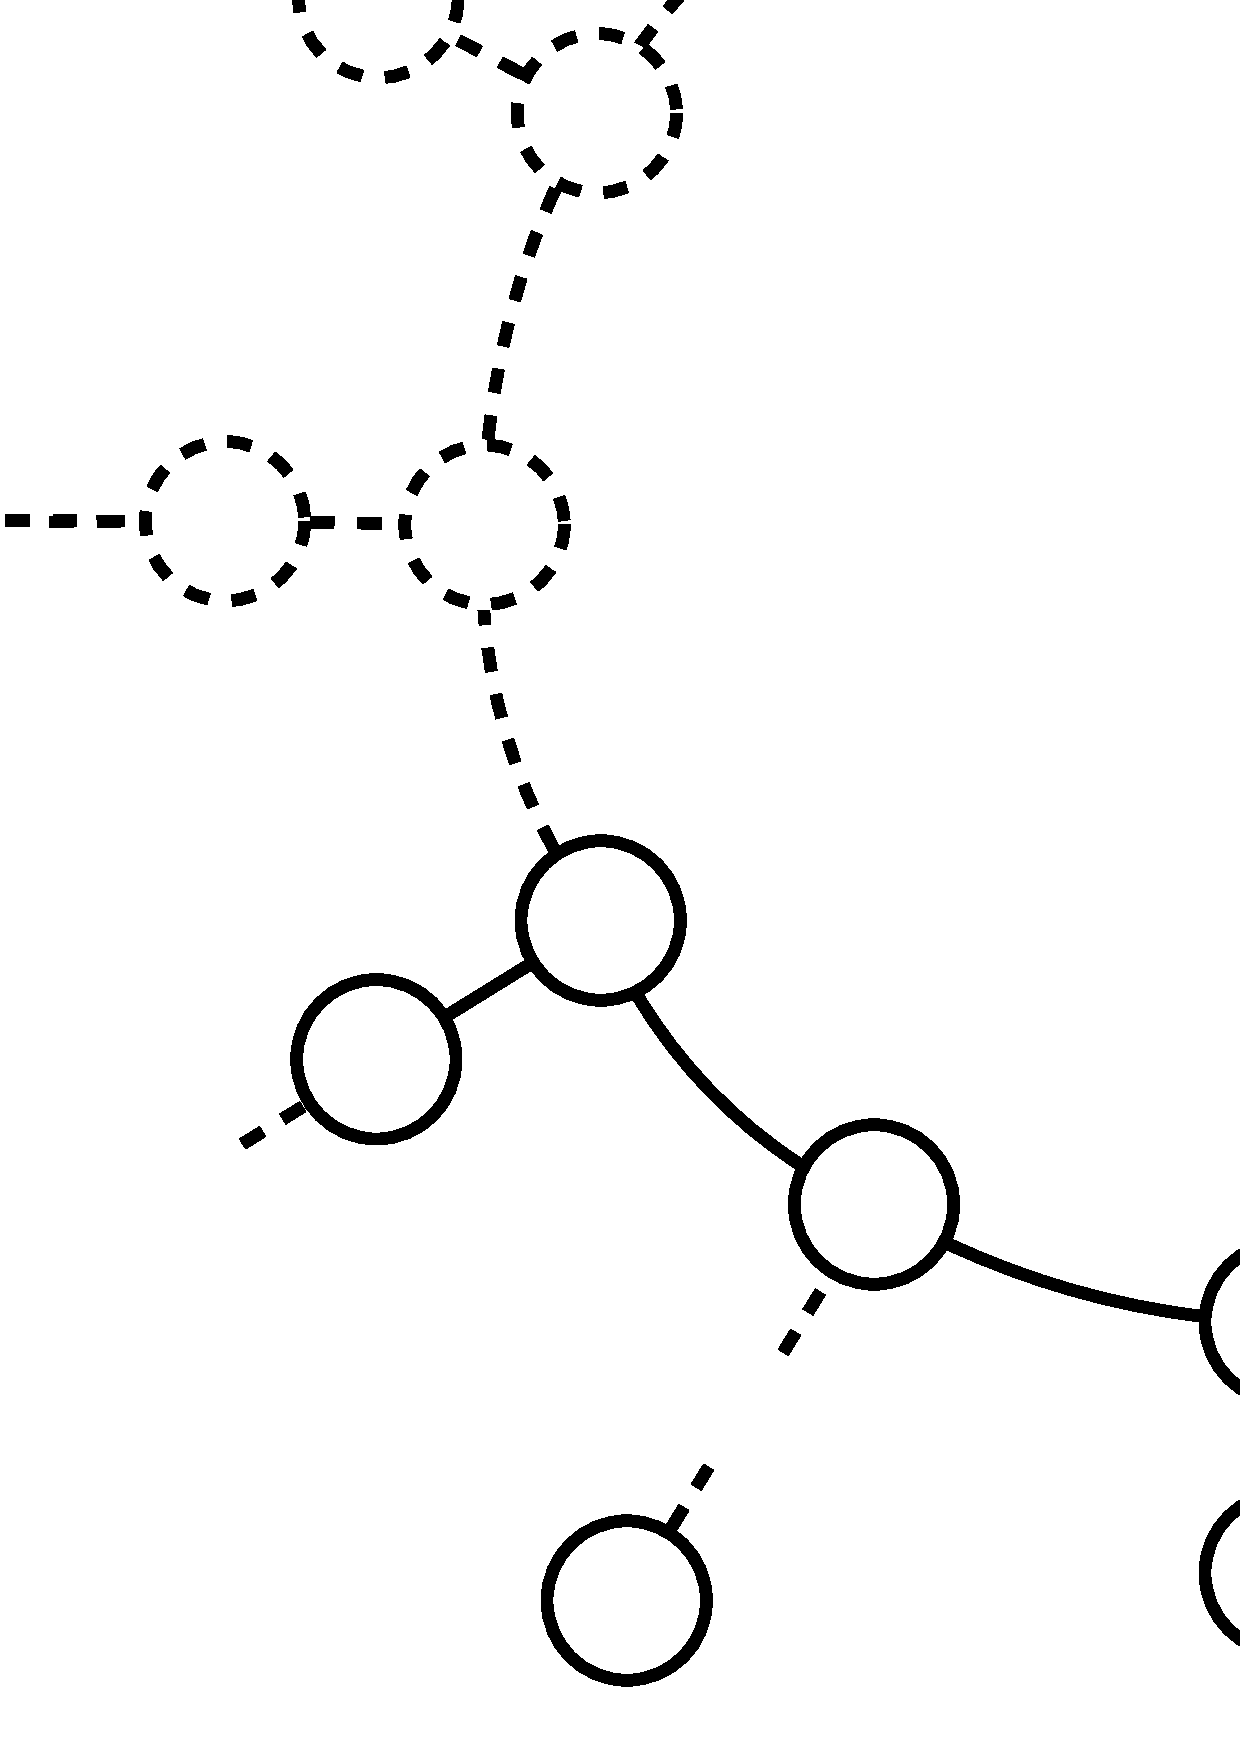
\includegraphics[width=170pt]{bilder/sonne2.pdf}
%  \caption{Der Sonnengraph $S_{2n,2}$}
%	\label{Bild2}
%\end{minipage}
%\end{figure}
%\vspace{-7mm}
\begin{proof}[Beweis:]~
Für den ersten Knoten in der metrischen Basis gibt es $(k-1)\cdot n$ Möglichkeiten, aber nur $n$ unterschiedliche Fälle. Denn wird der erste Knoten aus einem Strahl aufgenommen, so gilt nach Lemma \ref{bifur}, dass der Strahlursprung als Element der metrischen Basis betrachtet werden kann.\\
\vspace{-8mm}
 \begin{figure}[h!]
		\centering
 		 \includegraphics[width=100pt]{bilder/gbsbspsonne2glr.pdf}
   \caption{Ein $C_{n}-Blatt$ mit zwei Knoten in der metrischen Basis, welche die Bedingung von Lemma \ref{Bifurnachbar} erfüllen}
  	 \end{figure}
\vspace{-4mm}
  	 ~\linebreak
Der zweite Knoten muss die Bedingung vom Lemma \ref{Bifurnachbar} erfüllen. Es bleiben noch genau drei mögliche Knoten $v_{\frac{n}{2}}$, $v_{\frac{n-1}{2}}$ und $v_{\frac{n+1}{2}}$ als zweiter Ankerknoten.\\ 
Der Knoten $v_{\frac{n}{2}}$ kann nicht aufgenommen werden, da zwei gegenüberliegende Knoten einen Kreis gerader Länge nicht trennen.\\
Durch die Wahl von $v_{\frac{n-1}{2}}$ oder $v_{\frac{n+1}{2}}$ entstehen mindestens zwei Markierungen der Form $a/b$ und $a+1/b+1$ auf dem Kreis. Da jeder Knoten ein Strahlursprung ist, gibt es in dem Graphen einen weiteren Knoten mit der Markierung $a+1/b+1$. Zur Veranschaulichung wird der Graph $S_{6,2}$ betrachtet.
\begin{figure}[h!]
		\centering
 		 \includegraphics[width=120pt]{bilder/bspsonne6.pdf}
   \caption{Ein markierter $S_{6,2}$ mit zwei Knoten in der MB}
  	 \end{figure}
\end{proof}
%\begin{proof}[Beweis:]
%\begin{figure}[h!]
%		\centering
% 		 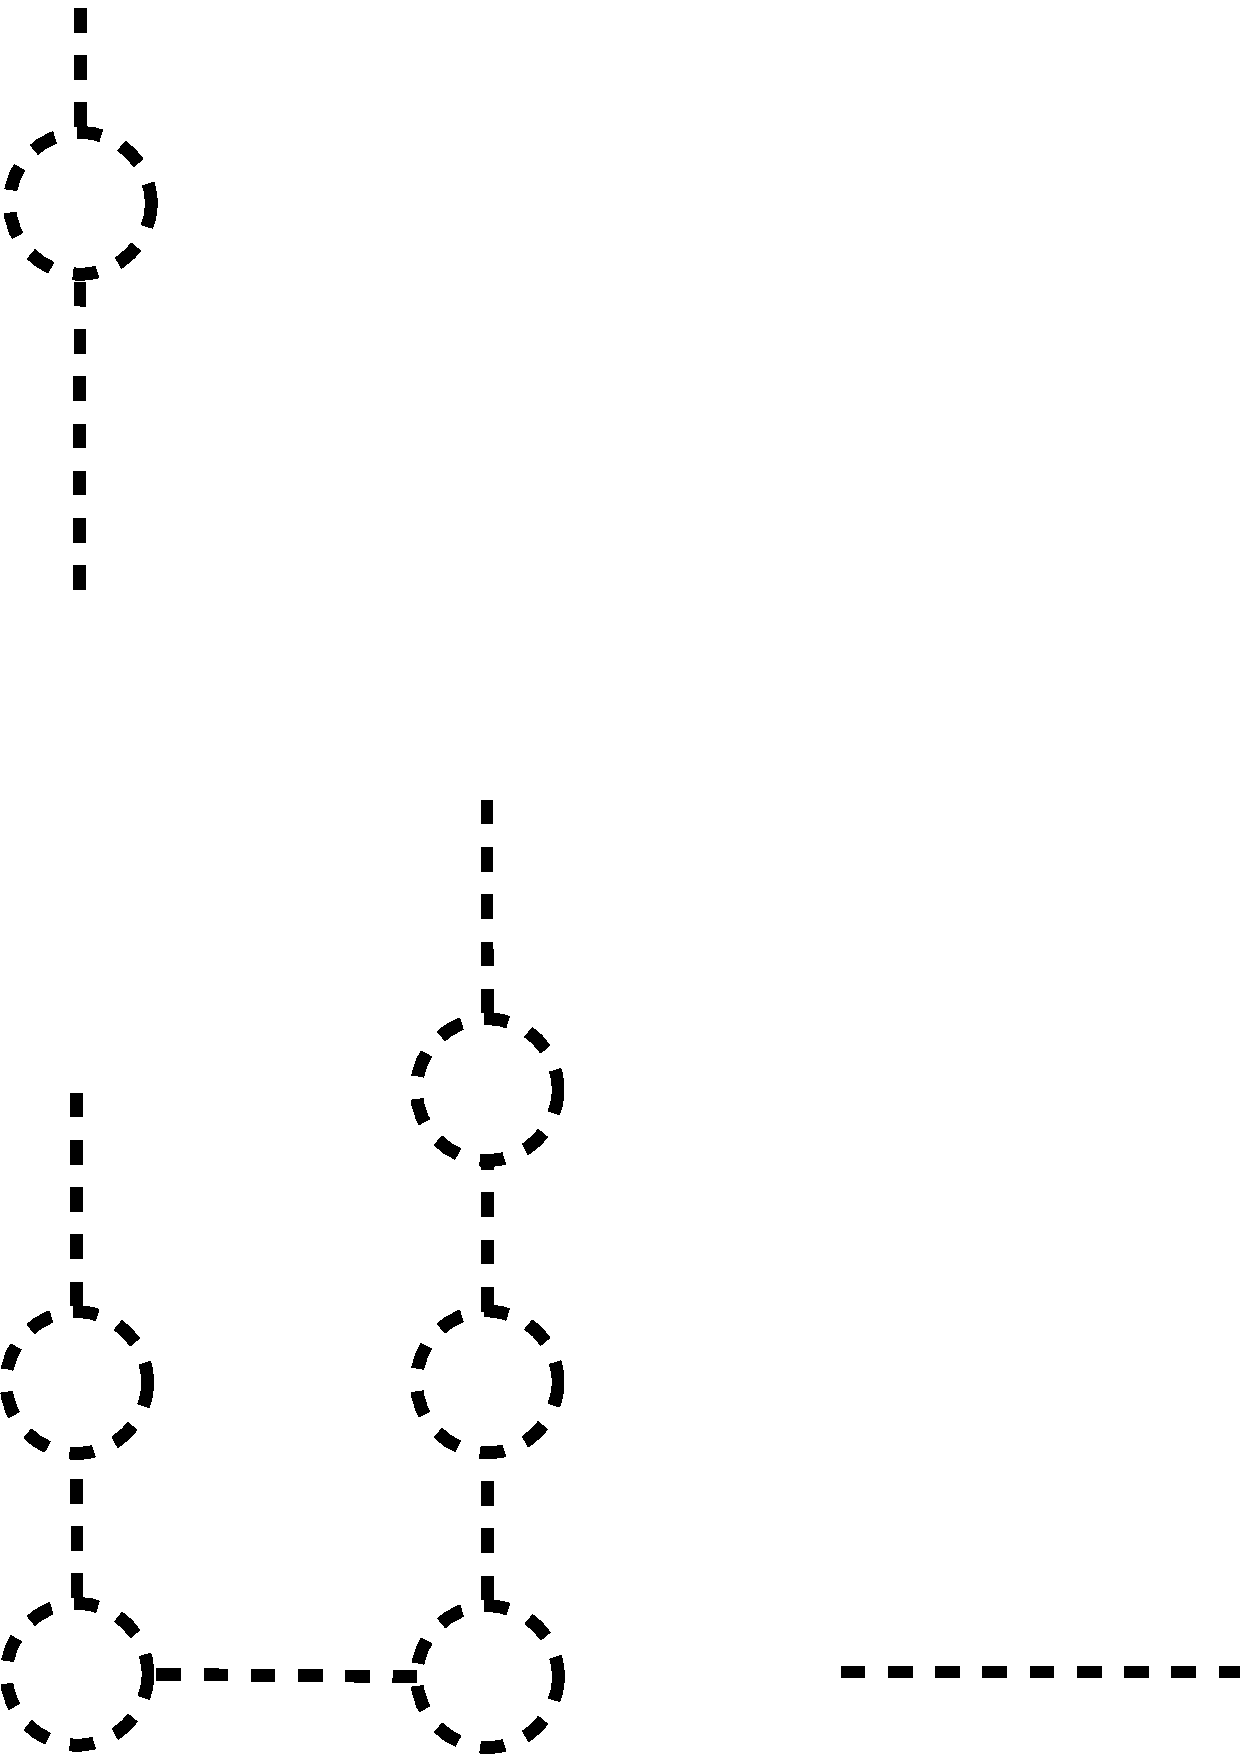
\includegraphics[width=430pt]{bilder/sonne1.pdf}
%   \caption{Ein $C_{n}-Blatt$ wird durch zwei Knoten getrennt}
%  	 \end{figure}
%Jeder Knoten auf einem Strahl hat eine $a+x/b+x$ Markierung mit $0 \leq x \leq k$ und $a/b$ die Markierung des Strahlursprung auf dem Kreis $C_n$.
%\end{proof}

\subsection{Metrische Dimension unvollständiger Sonnengraphen}  	
\label{chap_usonne} 
\begin{defi}{\textbf{(Unvollständiger Sonnengraph $S'_{n,k}$)}}\\
Sei ein Kreis $C_n$ für $n \geq 3$ mit der Knotenmenge $|V|=\{ c_1, \ldots , c_n \}$ und $n'$ Weggraphen $P_{k'}$ mit $1 \leq n' \leq n-1$ für $2 \leq k' \leq k$ gegeben. Die Knoten mit Grad eins auf dem $i-$ten Weg werden als $v_{i,1}$ und $v_{i,k-1}$ bezeichnet. Durch das Hinzufügen von $n'$ neuen Kanten der Form $\{v_{i,1},c_i\}$ für $1 \leq i \leq n$ ensteht der zusammenhängende Sonnengraph $S'_{n',k'}$. Gibt es mindestens zwei Strahlen mit unterschiedlicher Länge, so wird der unvollständige Sonnengraph als $S'_n$ bezeichnet. 
\end{defi}
\begin{lem}
Jeder unvollständige Sonnengraph ist ein Teilgraph eines Sonnengraphen und wird von dessen metrische Basis getrennt. Sind die Strahlen mit den Ankerknoten in dem unvollständigen Sonnengraphen nicht vorhanden, so können die Strahlurprungsknoten als Ankerknoten verwendet werden.
\end{lem}
\begin{proof}[Beweis:]

\end{proof}
\begin{satz}
\label{schrankenunvsg}
Für die metrische Dimension eines unvollständigen Sonnengraphen $S'_{n}$ gilt:
$$\beta(C_n) \leq \beta(S'_{n})\leq \beta(S_{n})$$
\end{satz}
\begin{proof}[Beweis:]
Um einen unvollständigen Sonnengraphen aus einem Kreis $C_n$ zu erhalten wird mindestens ein neuer Knoten erzeugt und mit genau einem Knoten in dem Graphen $C_n$ verbunden. Dieser Vorgang wird wiederholt bis der gewünschte unvollständige Graph erzeugt ist. Um einen Sonnengraphen $S_{n}$ aus einem unvollständigen Sonnengraphen zu erhalten wird mindestens ein Knoten hinzugefügt und mit genau einer Kante verbunden.% Sei $k$ die Anzahl der neu eingefügten Knoten zur Entstehung von dem $S_n$. 
Nach Lemma \ref{dist} gilt für die metrische Dimension:
$$\beta(C_n)  \leq \beta(S'_{n}) \leq \beta(C_n) +1 \text{ und } \beta(S'_{n}) \leq \beta(S_n) \leq \beta(S'_{n})+1$$
\end{proof}
\begin{bem}
Nach Satz \ref{schrankenunvsg} gilt für $n=2k+1$ für $k \in \mathbb{N}$: $$2=\beta(C_n) \leq \beta(S'_{n,k})\leq \beta(S_{n,k})=2$$
Daraus folgt, dass die metrische Dimension eines unvollständigen Sonnengraphen $S'_{n,k}$ mit $n=2k+1$ für $k \in \mathbb{N}$ zwei ist.\\
Für die metrische Dimension für $n=2k+2$ für $k \in \mathbb{N}$ gilt: $$2=\beta(C_n) \leq \beta(S'_{n,k})\leq \beta(S_{n,k})=3$$
Daraus folgt, dass die metrische Dimension eines unvollständigen Sonnengraphen $S'_{n,k}$ mit $n=2k+2$ für $k \in \mathbb{N}$ entweder zwei oder drei ist. Um die metrische Dimension genau zu bestimmen werden $\frac{n}{2}$ unterschiedliche Fälle betrachtet.
\end{bem}
\begin{table}[htp]
\centering
 \renewcommand{\arraystretch}{2}
\begin{tabularx}{\textwidth}{||c|c||}
\hline\hline
\vspace{0.3mm}
1. Fall& \multirow{3}{121mm}{$\frac{n}{2}-2$ benachbarte Knoten ohne Strahlen}\\
\cline{1-1}
\vspace{-6mm}
&\\
	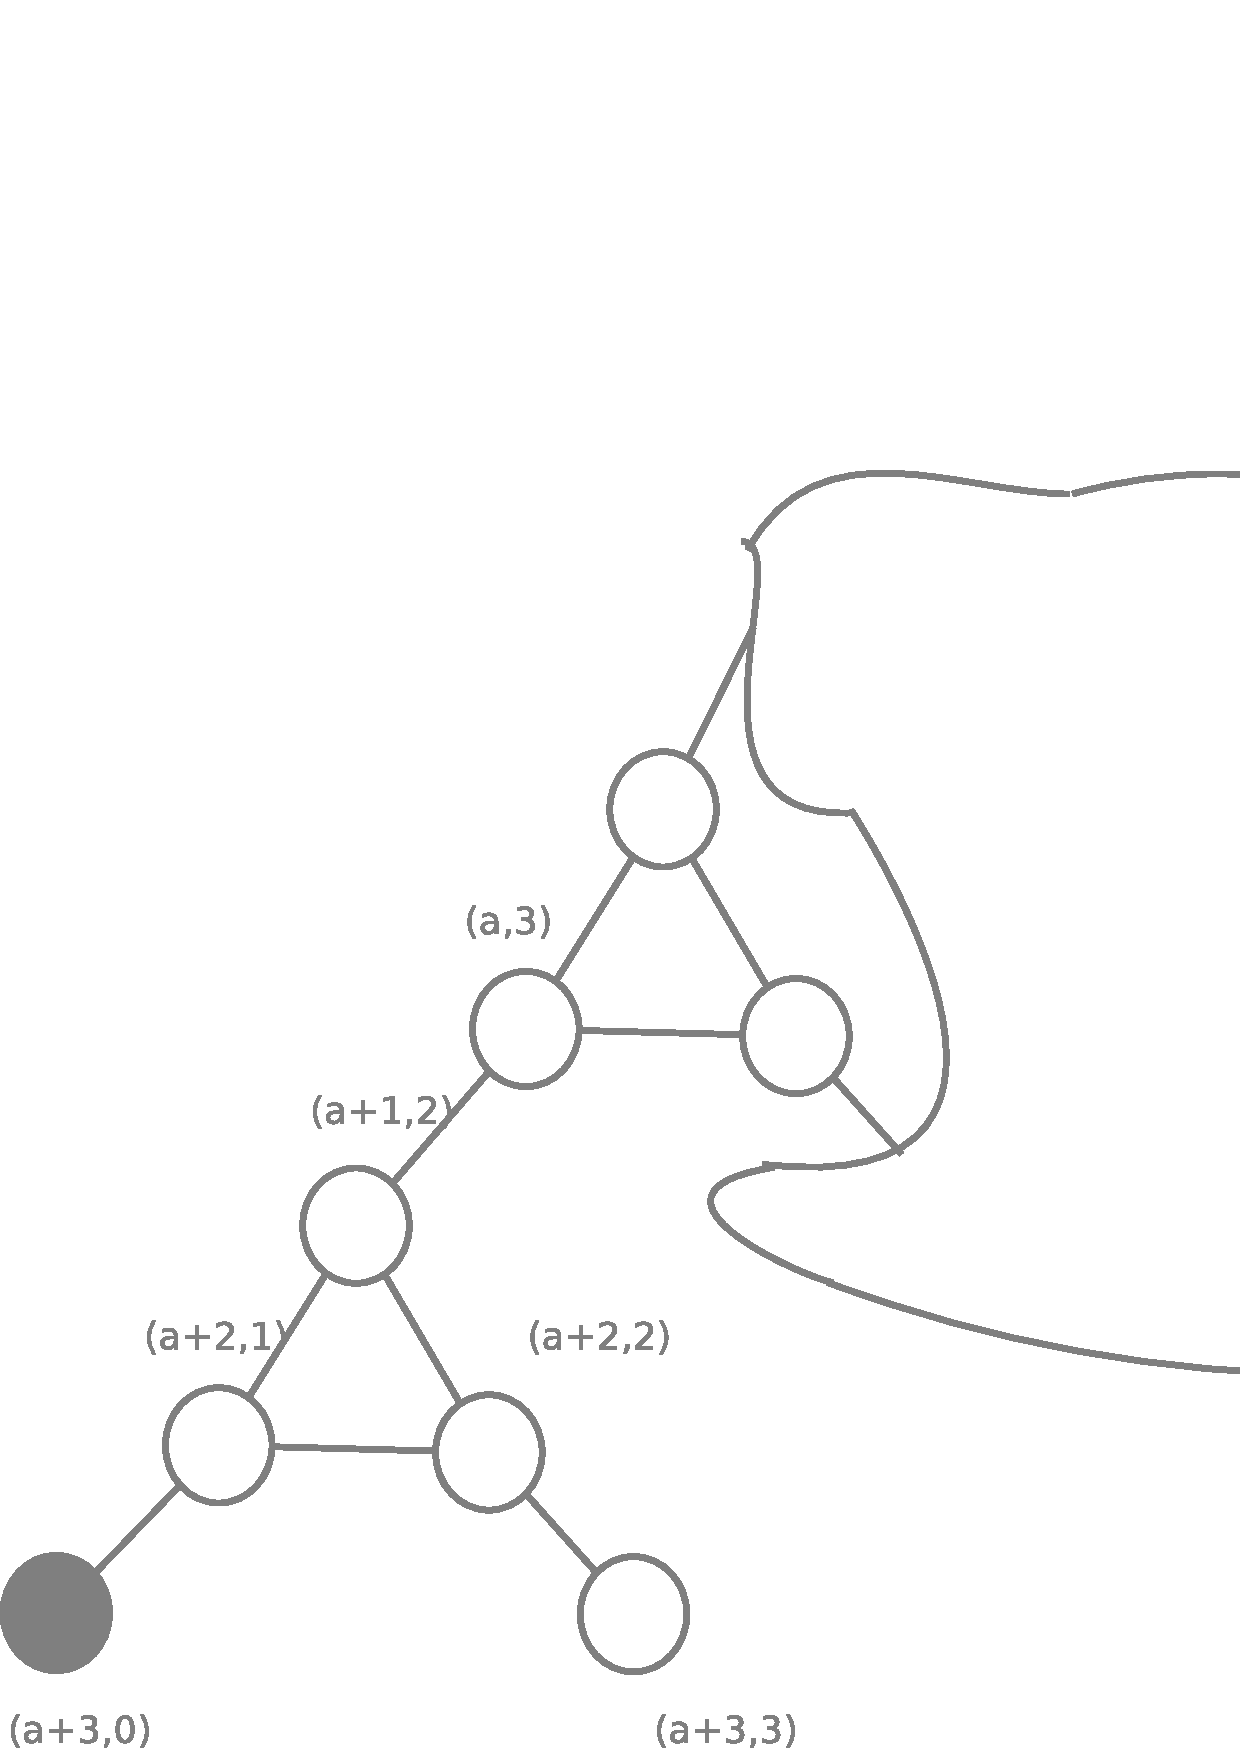
\includegraphics[width=50pt]{bilder/fall1.pdf}&\\
\hline\hline
\vspace{0.3mm}
2. Fall&\multirow{3}{121mm}{$2$ antipodale Knoten ohne Strahlen, $2$ Knoten mit/ohne Strahlen und $\frac{n}{2}-3$ Knoten ohne Strahlen der Länge $2$}\\
\cline{1-1}
\vspace{-6mm}&\\
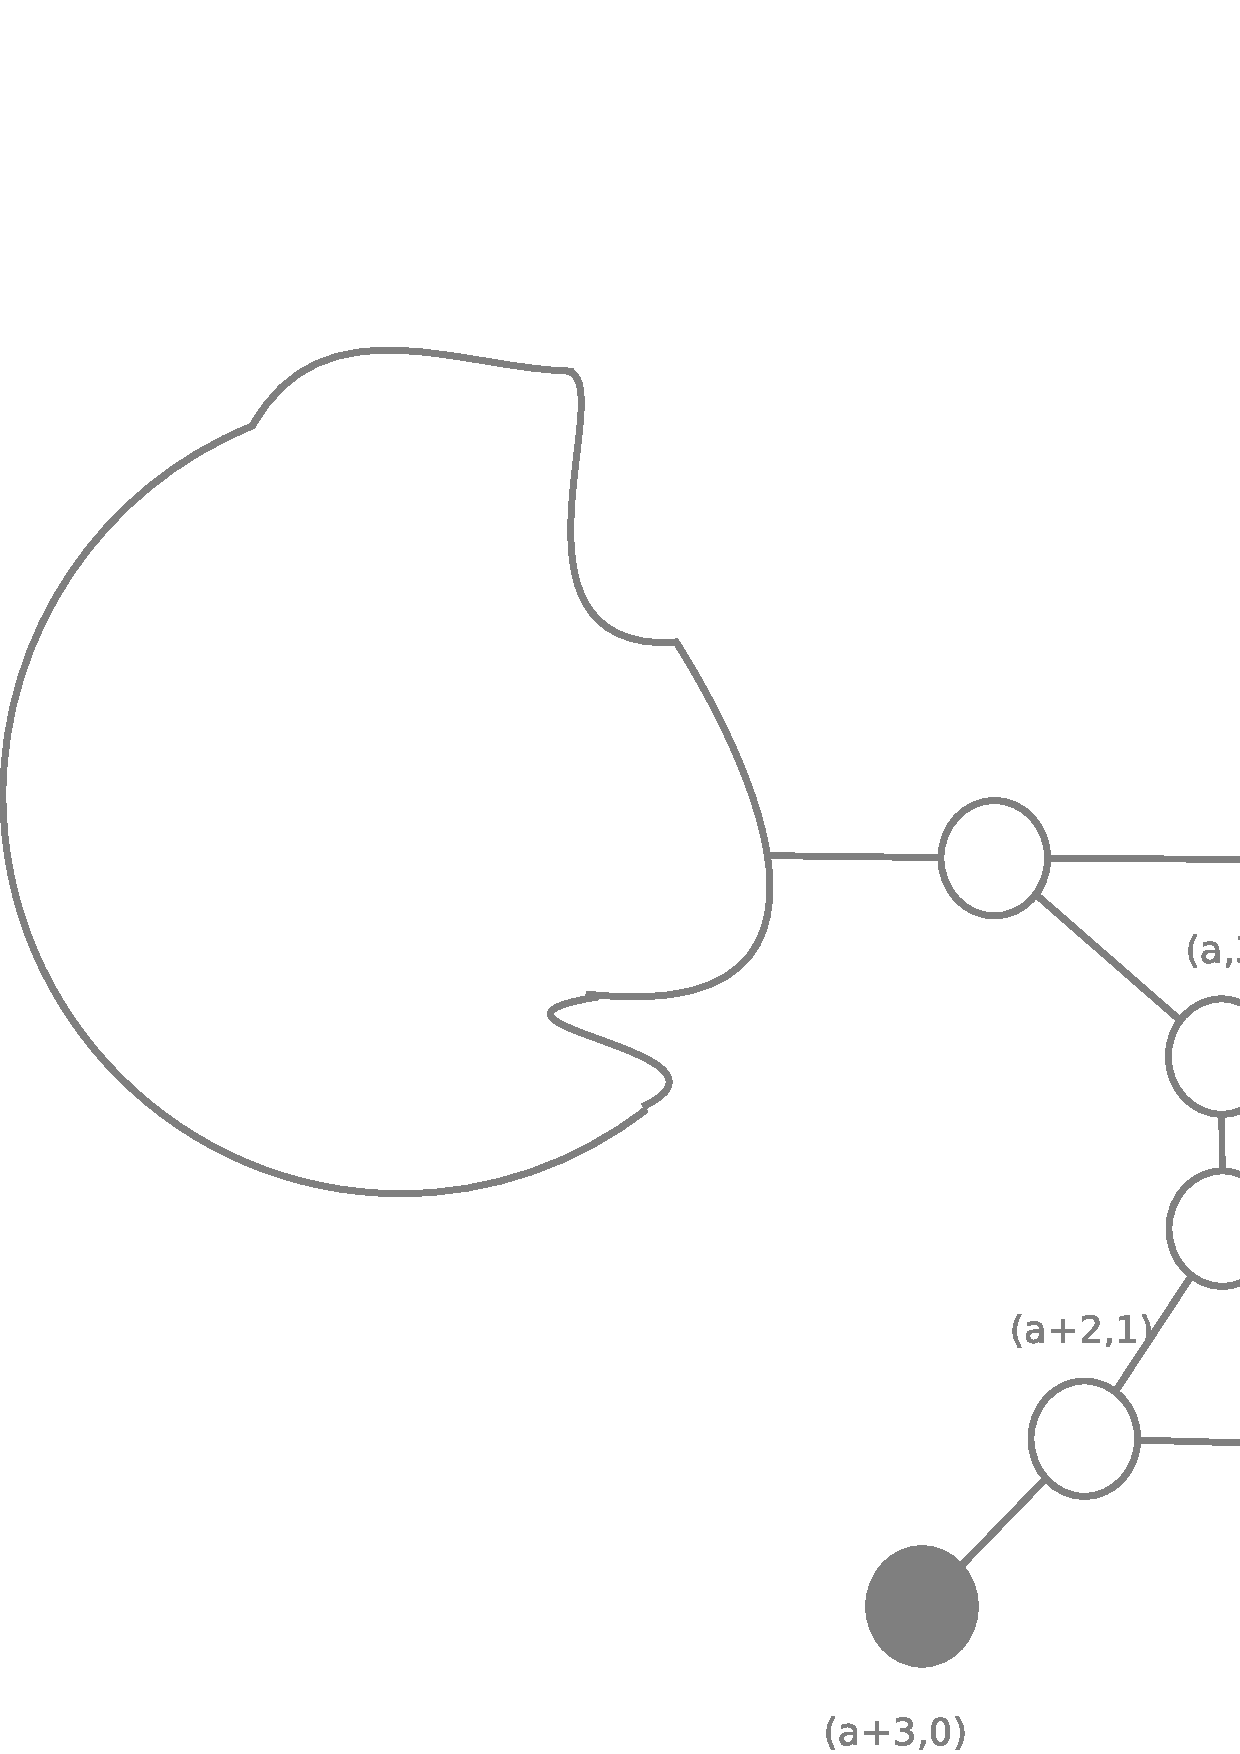
\includegraphics[width=50pt]{bilder/fall2.pdf}&\\
\hline\hline
\vspace{0.3mm}
3. Fall&\multirow{3}{121mm}{ $4$ antipodale Knoten ohne Strahlen (je $2$), $2$ Knoten mit/ohne Strahlen und $\frac{n}{2}-4$ Knoten ohne Strahlen der Länge $3$}\\
\cline{1-1}
\vspace{-6mm}&\\
\includegraphics[width=50pt]{bilder/fall3.pdf}&\\
\hline\hline
$\cdot$ &  $\cdot$\\
$\cdot$ &  $\cdot$\\
$\cdot$ &  $\cdot$\\
\hline\hline
\vspace{0.3mm}
$\frac{n}{2}-2$. Fall&\multirow{3}{121mm}{$n-2$ antipodale Knoten ohne Strahlen (je $\frac{n}{2}-1$), $2$ Knoten mit/ohne Strahlen und $1$ Knoten ohne Strahlen der Länge $\frac{n}{2}-1$}\\
\cline{1-1}
\vspace{-6mm}&\\
\includegraphics[width=50pt]{bilder/fall4.pdf}&\\
\hline\hline
\vspace{0.3mm}
$\frac{n}{2}-1$. Fall&\multirow{3}{121mm}{$n-4$ antipodale Knoten ohne Strahlen (je $\frac{n}{2}-2$)}\\
\cline{1-1}
\vspace{-6mm}&\\
\includegraphics[width=50pt]{bilder/falln2-1.pdf}&\\
\hline\hline
\end{tabularx}
\caption{Unvollständige Sonnen mit metrischer Dimension zwei}
\label{fallunterscheidungungeradesonnen2md}
\end{table}
%%%%%%%%%%%%%%%%%%%%%%%%%%%%%%%%%%%%%%%%%%%%%%%%%%%%%%%%%%%%%%%%%%%%%%%%%%%%%%%%%%%%%%%%%%%%%%%%%%%%%%%%%%%%%%%%%%%%%%%%%%%%%%%%
\newpage
\begin{comment}
\section{Vollständigen Graphen mit Strahlen $K^s_{n,i}$}
\section{Der erweiterte Gittergraph}
\section{Eine Erweiterung der Radgraphen $W_{n,i}$}
\end{comment}
%%%%%%%%%%%%%%%%%%%%%%%%%%%%%%%%%%%%%%%%%%%%%%%%%%%%%%%%%%%%%%%%%%%%%%%%%%
%%%%%%%%%%%%%%%%%%%%%%%%%%%%%%% ENDE TEXTTEIL %%%%%%%%%%%%%%%%%%%%%%%%%%%%
%%%%%%%%%%%%%%%%%%%%%%%%%%%%%%%%%%%%%%%%%%%%%%%%%%%%%%%%%%%%%%%%%%%%%%%%%%
%\vspace*{\fill}
%\pagebreak
%\printindex
\end{document}
